\solutionset

\begin{enumerate}

\item {\bf A Simple Protostellar Evolution Model.}

\begin{enumerate}

\item The star is a polytrope, and for a polytrope of index $n$ the gravitational energy is (e.g., see \citealt{kippenhahn94a})
\begin{displaymath}
\mathcal{W} = -\frac{3}{5-n} \frac{G M^2}{R}.
\end{displaymath}
The virial theorem tells us that the thermal energy is half the absolute value of the potential energy, so
\begin{displaymath}
\mathcal{T} = \frac{3}{2(5-n)} \frac{G M^2}{R}.
\end{displaymath}
Finally, the change in internal energy associated with dissociation, ionization, and deuterium burning is $(\psi_I  + \psi_M - \psi_D) M$. Note the opposite signs: $\psi_I$ and $\psi_M$ are positive, meaning that the final state (ionized, atomic) is higher energy than the initial one, while $\Psi_D$ is negative, indicating that the final state (all the deuterium converted to He) is a lower energy state than the initial one. Putting this all together, the total energy of the star is
\begin{displaymath}
\mathcal{E} = -\frac{3}{2(5-n)} \frac{G M^2}{R} + (\psi_I  + \psi_M - \psi_D) M.
\end{displaymath}

\item First we can compute the time rate of change of the star's energy,
\begin{displaymath}
\dot{\mathcal{E}} = \frac{3}{2(5-n)} \frac{GM}{R} \left(M\frac{\dot{R}}{R} - 2\dot{M}\right) + (\psi_I + \psi_M-\psi_D) \dot{M}.
\end{displaymath}
Now consider conservation of energy. The star's luminosity $L$ represents the rate of change of the energy "at infinity", i.e., the energy removed from the system. Since the total energy of the star plus infinity must remain constant, we require that $\dot{\mathcal{E}} + L = 0$. Writing down this condition and solving for $\dot{R}$, we obtain
\begin{displaymath}
\dot{R} = 2 R \frac{\dot{M}}{M} - \frac{2(5-n)}{3} \frac{R^2}{G M^2}\left[(\psi_I+\psi_M-\psi_D) \dot{M}+L\right]
\end{displaymath}
It is convenient to divide through by $\dot{M}$ in order to recast this as an equation for the evolution of $R$ with $M$:
\begin{displaymath}
\frac{dR}{dM} = 2 \frac{R}{M} - \frac{2(5-n)}{3} \frac{R^2}{G M^2}\left(\psi_I+\psi_M-\psi_D+\frac{L}{\dot{M}}\right).
\end{displaymath}
If we further divide by $R/M$ on both sides, we obtain
\begin{displaymath}
\frac{d\ln R}{d\ln M} = 2 - \frac{2(5-n)}{3} \frac{R}{G M}\left(\psi_I+\psi_M-\psi_D+\frac{L}{\dot{M}}\right).
\end{displaymath}
Next, we must compute the total luminosity, which contains contributions from the star's intrinsic, internal luminosity, and from the accretion luminosity. Since the star is on the Hayashi track, we can compute the intrinsic luminosity by taking its effective temperature to be fixed at $T_H$. Thus the total luminosity is
\begin{displaymath}
L = L_{\rm acc} + L_H = f_{\rm acc} \frac{G M \dot{M}}{R} + 4\pi R^2 \sigma T_H^4.
\end{displaymath}
Substituting this in, we have
\begin{displaymath}
\frac{d\ln R}{d\ln M} = 2 - \frac{2(5-n)}{3} \left[f_{\rm acc} + \left(\frac{R}{G M}\right)\left(\psi_I+\psi_M -\psi_D + \frac{4\pi R^2\sigma T_H^4}{\dot{M}}\right)\right].
\end{displaymath}
This is our final evolution equation.

\item The ODE can be integrated by standard techniques. Below is an example python program to do so, and plot the result:
\begin{verbatim}
import numpy as np
import matplotlib.pyplot as plt
from scipy.integrate import odeint

# Define some constants in cgs
G = 6.67e-8
eV = 1.6e-12
amu = 1.66e-24
sigma = 5.67e-5
Msun = 1.99e33
Rsun = 6.96e10
Lsun = 3.83e33
yr = 365.25*24.*3600.

# Problem parameters
psiI = 13.6*eV/amu
psiM = 2.2*eV/amu
psiD = 100*eV/amu
tH = 3500.0

# Default parameters
n = 1.5
facc = 0.75
Mdot = 1e-5*Msun/yr

# Define the derivative function
def dlnRdlnM(lnR, lnM, n=n, facc=facc, Mdot=Mdot):
    R = np.exp(lnR)
    M = np.exp(lnM)
    return(2.0-2.0*(5.0-n)/3.0 *
           (facc+(R/(G*M))*
            (psiI+psiM-psiD+
             4.0*np.pi*R**2*sigma*tH**4/Mdot)))

# Integrate
lnM = np.log(np.logspace(-2, 0, 500)*Msun)
lnR = odeint(dlnRdlnM, np.log(2.5*Rsun), lnM,
             args=(n, facc, Mdot))
R = np.exp(lnR[:,0])
M = np.exp(lnM)
             
# Get luminosity
L = facc*G*M*Mdot/R + 4.0*np.pi*R**2*sigma*tH**4

# Plot radius
p1,=plt.plot(M/Msun, R/Rsun, 'b', lw=2)
plt.xscale('log')
plt.xlabel(r'$M/M_\odot$')
plt.ylabel(r'$R/R_\odot$')

# Plot luminosity
plt.twinx()
p2,=plt.plot(M/Msun, L/Lsun, 'r', lw=2)
plt.ylabel(r'$L/L_\odot$')
plt.legend([p1,p2], ['Radius', 'Luminosity'],
           loc='lower right')
\end{verbatim}
\begin{marginfigure}
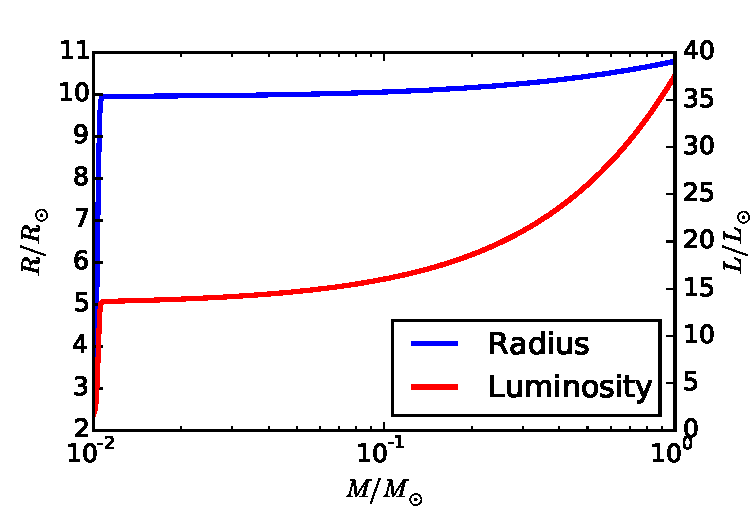
\includegraphics[width=\linewidth]{hw5sol1}
\caption[Solution to problem set~\thesolutionset, problem~\theenumi\theenumii]{
\label{fig:hw5sol1}
Radius (blue) and luminosity (red) for the simple protostellar evolution model.
}
\end{marginfigure}
The resulting output is shown as Figure \ref{fig:hw5sol1}. Note that the radius is too large by a factor of $\sim 3$ compared to more sophisticated models, mainly due to the incorrect assumption that all the accreted deuterium burns as quickly as it accretes. In reality the D luminosity should be significantly lower, because D burning lasts longer than accretion.

\item This problem can be solved using the same basic structure as the previous part. The derivative of radius with respect to mass now becomes
\begin{eqnarray*}
\frac{d\ln R}{d\ln M} & = & 2 - \frac{2(5-n)}{3} \left[f_{\rm acc} + \left(\frac{R}{G M}\right) \cdot \right.
\\
& & \qquad \left.\left(\psi_I+\psi_M -\psi_D + \frac{\max[4\pi R^2\sigma T_H^4, \lsun (M/\msun)^3]}{\dot{M}}\right)\right].
\end{eqnarray*}
This can be integrated via a simple python program as in the previous part:
\begin{verbatim}
# Define the derivative function for the second part
def dlnRdlnM2(lnR, lnM, n=n, facc=facc, Mdot=Mdot):
    R = np.exp(lnR)
    M = np.exp(lnM)
    LH = 4.0*np.pi*R**2*sigma*tH**4
    Lstar = Lsun*(M/Msun)**3
    return(2.0-2.0*(5.0-n)/3.0 *
           (facc+(R/(G*M))*
            (psiI+psiM-psiD+np.maximum(Lstar,LH)/Mdot)))

# Integrate
Mdot2 = 1.0e-4*Msun/yr
lnM2 = np.log(np.logspace(-2, np.log10(50), 500)*Msun)
lnR2 = odeint(dlnRdlnM2, np.log(2.5*Rsun), lnM2,
              args=(3.0, facc, Mdot2))
R2 = np.exp(lnR2[:,0])
M2 = np.exp(lnM2)

# Get luminosity
L2 = facc*G*M*Mdot/R + np.maximum(
    4.0*np.pi*R2**2*sigma*tH**4,
    Lsun*(M2/Msun)**3)

# Plot radius
clf()
p1,=plt.plot(M2/Msun, R2/Rsun, 'b', lw=2)
plt.xlabel(r'$M/M_\odot$')
plt.ylabel(r'$R/R_\odot$')

# Plot luminosity
plt.twinx()
p2,=plt.plot(M2/Msun, L2/Lsun, 'r', lw=2)
plt.ylabel(r'$L/L_\odot$')
plt.yscale('log')
plt.xlim([0,50])
plt.legend([p1,p2], ['Radius', 'Luminosity'], 
           loc='center right')
\end{verbatim}
\begin{marginfigure}
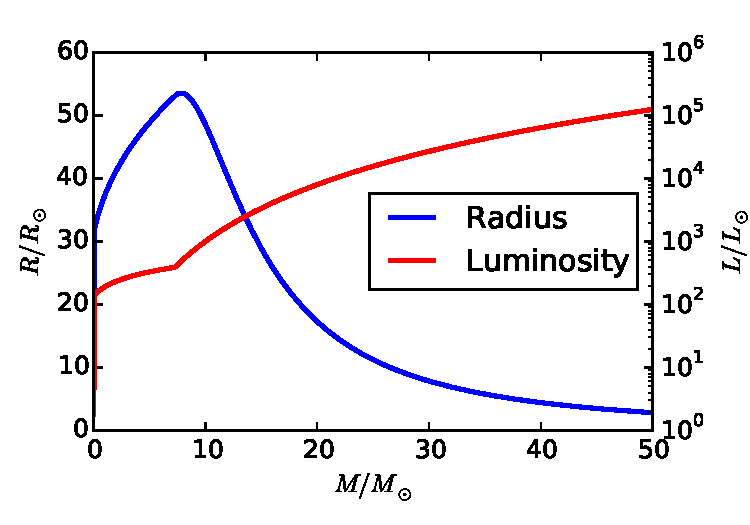
\includegraphics[width=\linewidth]{hw5sol2}
\caption[Solution to problem set~\thesolutionset, problem~\theenumi\theenumii]{
\label{fig:hw5sol2}
Radius (blue) and luminosity (red) for the simple protostellar evolution model for a massive star.
}
\end{marginfigure}
The resulting output is shown as Figure \ref{fig:hw5sol2}.

\end{enumerate}

\item {\bf Disk Dispersal by Photoionization.}

\begin{enumerate}

\item The gas will escape when the sound speed becomes comparable to the escape speed from the star. Thus
\begin{eqnarray*}
c_s & \approx & \sqrt{\frac{2 G M_*}{r_g}}\\
r_g & \approx & \frac{2 G M_*}{c_s^2} = \frac{2 G M_* \mu}{k_B T}
\end{eqnarray*}
The mean particle mass depends on whether the helium is ionized or not, but for a relatively cool star like a T Tauri star it is probably reasonable to assume that it is not, so the number of electrons equals the number of hydrogen atoms. The mean mass per particle for neutral hydrogen is $2.34\times 10^{-24}$ g, and by number hydrogen represents 93\% of all nuclei in the Milky Way, so the mean mass per particle in gas where the hydrogen is ionized is $\mu=1.2\times 10^{-24}$ g. Plugging this in gives a sound speed $c_s = 10.7$ km s$^{-1}$.

\item Ionization balance requires that recombinations equal ionizations. If the density is $n_0$ inside $r_g$, the recombination rate per unit volume is $\alpha^{(B)} n_0^2$, where $\alpha^{(B)}=2.59\times 10^{-13}$ cm$^{-3}$ s$^{-1}$ is the case B recombination coefficient, and this expression implicitly assumes that the gas is fully ionized. The recombination rate is simply this times the volume, so equating this with the ionization rate produced by the star give
\begin{eqnarray*}
\Phi & = & \frac{4}{3}\pi r_g^3 \alpha^{(B)} n_0^2 \\
n_0 & = & \sqrt{\frac{3\Phi}{4\pi \alpha^{(B)} r_g^3}} \\
& = & \sqrt{\frac{3\Phi k_B^3 T^3}{32\pi \alpha^{(B)} G^3 M_*^3 \mu^3}}
\end{eqnarray*}

\item The wind will have a density of $\sim n_0$ and will leave a velocity $\sim c_s$, and it will be lost from an area of order $r_g^2$. Thus an order of magnitude estimate for the wind mass flux is
\begin{eqnarray*}
\dot{M} & \sim & n_0 m_H c_s r_g^2 \\
& = & \sqrt{\frac{3\Phi r_g}{4\pi \alpha^{(B)}}} m_H c_s \\
& = & \sqrt{\frac{3\Phi G M_* m_H^2}{2\pi \alpha^{(B)}}}
\end{eqnarray*}

\item Plugging in the given numerical values gives $\dot{M} \sim 10^{-10}$ $\msun$ yr$^{-1}$. Thus it would take $\sim 100$ Myr to evaporate a $0.01$ $\msun$ star. This is much longer than the observed $\sim 2$ Myr lifetime of T Tauri disks. This indicates that photoionization by itself cannot the the primary disk removal mechanism. Instead, it is a plausible disk destruction mechanism only if it operates in tandem with some other mechanism, like accretion of the disk onto the star.

\end{enumerate}

\item {\bf Aerodynamics of Small Solids in a Disk.}

\begin{enumerate}

\item The force per unit mass in the radial direction that a parcel of gas of density $\rho$ experiences due to the combined effects of gas pressure and stellar gravity is
\begin{displaymath}
f_r = -\frac{G M}{r^2} - \frac{1}{\rho}\frac{\partial P}{\partial r} = -\frac{GM}{r^2} + \frac{n}{\rho}\frac{P}{r} = -\frac{GM}{r^2} + \frac{n c_s^2}{r}.
\end{displaymath}
This also gives the acceleration of the gas parcel toward the star. If we equate this with the centripetal acceleration required to maintain circular motion at velocity $v_g$, then we have
\begin{displaymath}
\frac{v_g^2}{r} = \frac{GM}{r^2} - \frac{n c_s^2}{r} = \frac{v_K^2}{r} - \frac{n c_s^2}{r},
\end{displaymath}
where $v_K = \sqrt{GM/r}$ is the Keplerian velocity. If we solve this for $v_g$ and subtract the result from $v_K$, then we have
\begin{eqnarray*}
\Delta v = v_K - v_g & = & v_K - \sqrt{v_K^2 - n c_s^2} \\
& = & v_K \left(1 - \sqrt{1 - \frac{n c_s^2}{v_K^2}}\right) \\
& \approx & \frac{n c_s^2}{2 v_K^2},
\end{eqnarray*}
where the last step results from taking the Taylor expansion of the square root term in the limit $nc_s^2 \ll v_K^2$, which is equivalent to the assumption that the deviation from Keplerian rotation is small.

\item The mass of the solid particle is $m_s = (4/3)\pi s^3 \rho_s$, so its momentum is $p = (4/3)\pi s^3 \rho_s v$. Dividing this by the drag force we have
\begin{displaymath}
t_s = \frac{p}{F_D} = \frac{s}{c_s}\frac{\rho_s}{\rho_d}.
\end{displaymath}
i.e.\ the stopping time is just the sound crossing time of the particle's radius multiplied by the ratio of solid density to gas density.

\item In the frame co-rotating with the gas, the dust particle experiences a net radial force which contains contributions from inward stellar gravity, outward centrifugal force, and outward drag force resisting inward motion. The total force is
\begin{eqnarray*}
F & = & -\frac{GM m_s}{r^2} + \frac{m_s v_g^2}{r} - \frac{4\pi}{3} s^2 \rho_d v c_s \\
& = & -\frac{v_K^2}{r} m_s + \left(\frac{v_K^2}{r} - \frac{n c_s^2}{r}\right) m_d - \frac{4\pi}{3} s^2 \rho_d v c_s \\
& = & \frac{c_s}{m_s} \left(-\frac{nc_s}{r} - \frac{v}{s}\frac{\rho_d}{\rho_s}\right),
\end{eqnarray*}
where $m_s = (4/3)\pi s^3 \rho_s$ is the mass of the solid. The terminal velocity of the grain is determined by the condition that the net force be zero, so if we set the right-hand side of this equation equal to zero and solve, we find that the terminal velocity is
\begin{displaymath}
v = -n c_s\frac{s}{r} \frac{\rho_s}{\rho_d}.
\end{displaymath}
The time required for the solid particle to drift into the star is roughly
\begin{displaymath}
t_{\rm drift} \approx \frac{r_0}{-v} = \frac{r_0^2}{n c_s s}\frac{\rho_d}{\rho_s},
\end{displaymath}

\item First let's evaluate the stopping time:
\begin{displaymath}
t_s = \frac{s}{c_s} \frac{\rho_s}{\rho_d} = \frac{s}{\sqrt{k_B T/\mu}} \frac{\rho_s}{\rho_d} = 2.1\times 10^4\mbox{ s}.
\end{displaymath}
The orbital period at 1 AU is $t_{\rm orb} = 1\mbox{ yr} = 3.1\times 10^7\mbox{ s}$, so we do have $t_s \ll t_{\rm orb}$. The timescale required for the particle to drift into the star is
\begin{displaymath}
t_{\rm drift} =  \frac{r_0^2}{n c_s s}\frac{\rho_d}{\rho_s} = 1.7\times 10^{11}\mbox{ s} = 5400\mbox{ yr}.
\end{displaymath}
This is much, much smaller than the inferred timescale of $\sim 1$ Myr for planet formation and disk dissipation.

\end{enumerate}

\end{enumerate}



